\documentclass{standalone}
\usepackage{tikz}
\usetikzlibrary{patterns}
\usetikzlibrary{positioning}
\usetikzlibrary{patterns, positioning}
\usetikzlibrary{shapes.misc}
\usepackage[outline]{contour}
\contourlength{1.5pt} 
\usepackage[sfdefault]{ClearSans}

\begin{document}
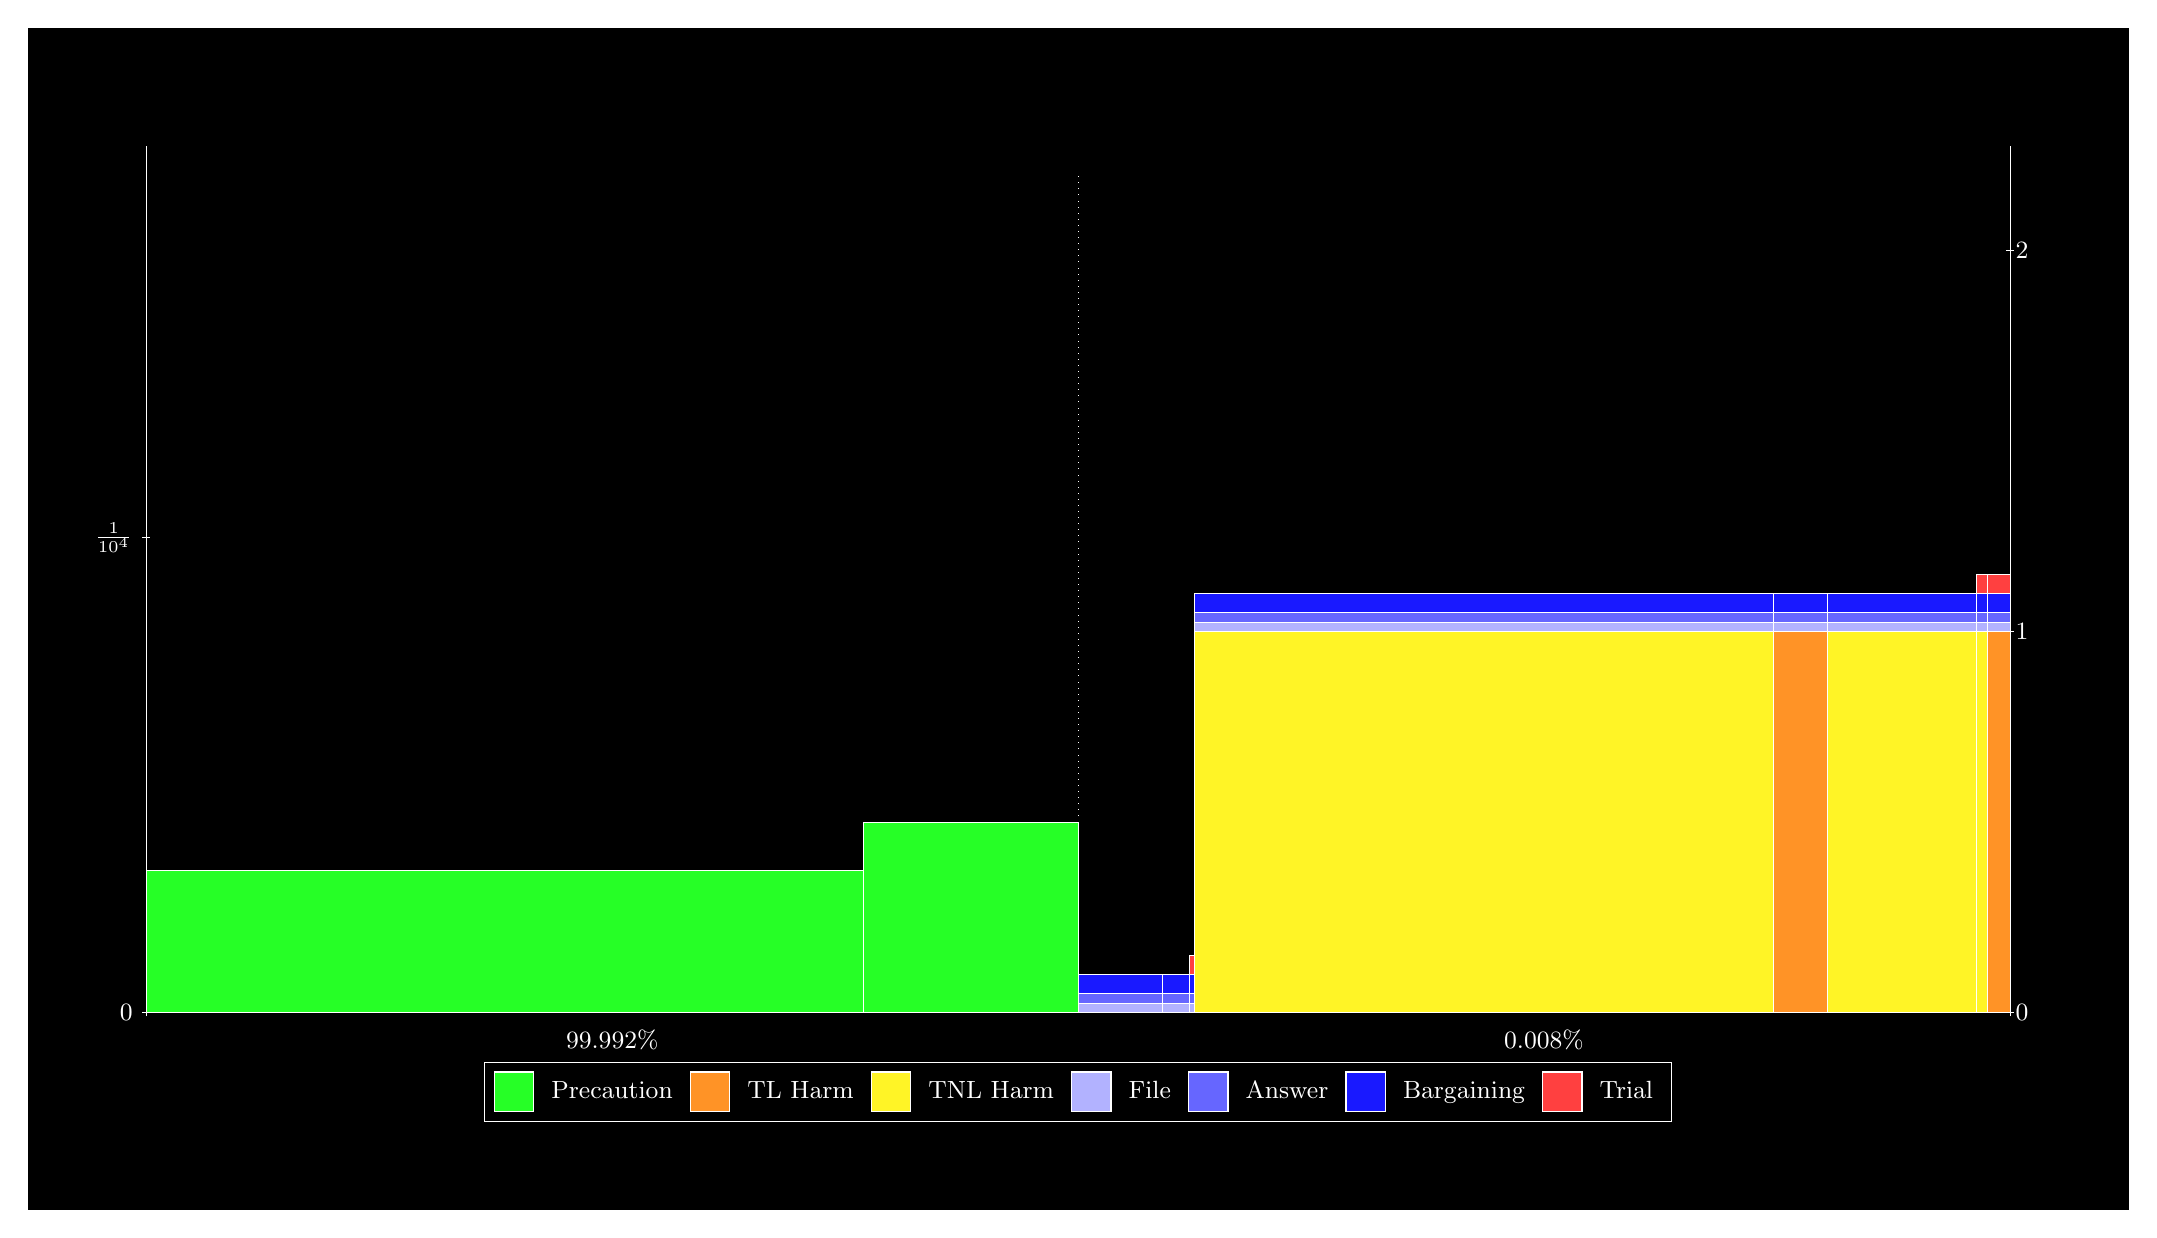
\begin{tikzpicture}
\draw[fill=black] (0,0) rectangle (26.667,15);
\draw[fill=green!85,draw=white,very thin] (1.5,2.5) rectangle (10.611,4.3089);
\draw[fill=green!85,draw=white,very thin] (10.611,2.5) rectangle (13.333,4.9118);
\draw[fill=green!85,draw=white,very thin] (13.333,2.5) rectangle (14.403,2.5001);
\draw[fill=blue!30,draw=white,very thin] (13.333,2.5001) rectangle (14.403,2.6211);
\draw[fill=blue!60,draw=white,very thin] (13.333,2.6211) rectangle (14.403,2.7421);
\draw[fill=blue!90,draw=white,very thin] (13.333,2.7421) rectangle (14.403,2.9841);
\draw[fill=green!85,draw=white,very thin] (14.403,2.5) rectangle (14.742,2.5002);
\draw[fill=blue!30,draw=white,very thin] (14.403,2.5002) rectangle (14.742,2.6212);
\draw[fill=blue!60,draw=white,very thin] (14.403,2.6212) rectangle (14.742,2.7422);
\draw[fill=blue!90,draw=white,very thin] (14.403,2.7422) rectangle (14.742,2.9842);
\draw[fill=green!85,draw=white,very thin] (14.742,2.5) rectangle (14.808,2.5001);
\draw[fill=blue!30,draw=white,very thin] (14.742,2.5001) rectangle (14.808,2.6211);
\draw[fill=blue!60,draw=white,very thin] (14.742,2.6211) rectangle (14.808,2.7421);
\draw[fill=blue!90,draw=white,very thin] (14.742,2.7421) rectangle (14.808,2.9841);
\draw[fill=red!75,draw=white,very thin] (14.742,2.9841) rectangle (14.808,3.2261);
\draw[fill=green!85,draw=white,very thin] (14.808,2.5) rectangle (22.168,2.5001);
\draw[fill=yellow!85,draw=white,very thin] (14.808,2.5001) rectangle (22.168,7.3399);
\draw[fill=blue!30,draw=white,very thin] (14.808,7.3399) rectangle (22.168,7.4609);
\draw[fill=blue!60,draw=white,very thin] (14.808,7.4609) rectangle (22.168,7.5819);
\draw[fill=blue!90,draw=white,very thin] (14.808,7.5819) rectangle (22.168,7.8239);
\draw[fill=green!85,draw=white,very thin] (22.168,2.5) rectangle (22.849,2.5001);
\draw[fill=orange!85,draw=white,very thin] (22.168,2.5001) rectangle (22.849,7.3399);
\draw[fill=blue!30,draw=white,very thin] (22.168,7.3399) rectangle (22.849,7.4609);
\draw[fill=blue!60,draw=white,very thin] (22.168,7.4609) rectangle (22.849,7.5819);
\draw[fill=blue!90,draw=white,very thin] (22.168,7.5819) rectangle (22.849,7.8239);
\draw[fill=green!85,draw=white,very thin] (22.849,2.5) rectangle (24.738,2.5002);
\draw[fill=yellow!85,draw=white,very thin] (22.849,2.5002) rectangle (24.738,7.3399);
\draw[fill=blue!30,draw=white,very thin] (22.849,7.3399) rectangle (24.738,7.4609);
\draw[fill=blue!60,draw=white,very thin] (22.849,7.4609) rectangle (24.738,7.5819);
\draw[fill=blue!90,draw=white,very thin] (22.849,7.5819) rectangle (24.738,7.8239);
\draw[fill=green!85,draw=white,very thin] (24.738,2.5) rectangle (24.881,2.5001);
\draw[fill=yellow!85,draw=white,very thin] (24.738,2.5001) rectangle (24.881,7.3399);
\draw[fill=blue!30,draw=white,very thin] (24.738,7.3399) rectangle (24.881,7.4609);
\draw[fill=blue!60,draw=white,very thin] (24.738,7.4609) rectangle (24.881,7.5819);
\draw[fill=blue!90,draw=white,very thin] (24.738,7.5819) rectangle (24.881,7.8239);
\draw[fill=red!75,draw=white,very thin] (24.738,7.8239) rectangle (24.881,8.0658);
\draw[fill=green!85,draw=white,very thin] (24.881,2.5) rectangle (25.167,2.5001);
\draw[fill=orange!85,draw=white,very thin] (24.881,2.5001) rectangle (25.167,7.3399);
\draw[fill=blue!30,draw=white,very thin] (24.881,7.3399) rectangle (25.167,7.4609);
\draw[fill=blue!60,draw=white,very thin] (24.881,7.4609) rectangle (25.167,7.5819);
\draw[fill=blue!90,draw=white,very thin] (24.881,7.5819) rectangle (25.167,7.8239);
\draw[fill=red!75,draw=white,very thin] (24.881,7.8239) rectangle (25.167,8.0658);
\draw[white,very thin] (1.5,2.5) -- (1.5,13.5);
\draw[white,very thin] (1.45,2.5) -- (1.55,2.5);
\node[font=\small,text=white, anchor=east] at (1.45, 2.5) {0};
\draw[white,very thin] (1.45,8.5296) -- (1.55,8.5296);
\node[font=\small,text=white, anchor=east] at (1.45, 8.5296) {$\frac{1}{10^{4}}$};

\draw[white,dotted,very thin] (13.333,2.83) -- (13.333,13.17);
\draw[white,very thin] (25.167,2.5) -- (25.167,13.5);
\draw[white,very thin] (25.117,2.5) -- (25.217,2.5);
\node[font=\small,text=white, anchor=west] at (25.117, 2.5) {0};
\draw[white,very thin] (25.117,7.3397) -- (25.217,7.3397);
\node[font=\small,text=white, anchor=west] at (25.117, 7.3397) {1};
\draw[white,very thin] (25.117,12.179) -- (25.217,12.179);
\node[font=\small,text=white, anchor=west] at (25.117, 12.179) {2};

\draw[white,very thin] (1.5,2.5) -- (25.167,2.5);
\draw[white,very thin] (1.5,2.45) -- (1.5,2.55);
\node[font=\small,text=white, anchor=north] at (1.5, 2.45) {};
\draw[white,very thin] (25.167,2.45) -- (25.167,2.55);
\node[font=\small,text=white, anchor=north] at (25.167, 2.45) {};

\node[font=\small,text=white,anchor=south] at (7.4167, 1.9) {99.992\%};
\node[font=\small,text=white,anchor=south] at (19.25, 1.9) {0.008\%};
\draw (13.3333,2.5) node (B) {};
\begin{scope}[align=center]
\matrix[scale=0.5,draw=white,below=0.5cm of B,nodes={draw},column sep=0.1cm]{
\node[rectangle,draw,minimum width=0.5cm,minimum height=0.5cm,fill=green!85]{}; & \node[draw=none,font=\small,text=white]{Precaution}; &
\node[rectangle,draw,minimum width=0.5cm,minimum height=0.5cm,fill=orange!85]{}; & \node[draw=none,font=\small,text=white]{TL Harm}; &
\node[rectangle,draw,minimum width=0.5cm,minimum height=0.5cm,fill=yellow!85]{}; & \node[draw=none,font=\small,text=white]{TNL Harm}; &
\node[rectangle,draw,minimum width=0.5cm,minimum height=0.5cm,fill=blue!30]{}; & \node[draw=none,font=\small,text=white]{File}; &
\node[rectangle,draw,minimum width=0.5cm,minimum height=0.5cm,fill=blue!60]{}; & \node[draw=none,font=\small,text=white]{Answer}; &
\node[rectangle,draw,minimum width=0.5cm,minimum height=0.5cm,fill=blue!90]{}; & \node[draw=none,font=\small,text=white]{Bargaining}; &
\node[rectangle,draw,minimum width=0.5cm,minimum height=0.5cm,fill=red!75]{}; & \node[draw=none,font=\small,text=white]{Trial}; \\\\
};\end{scope}

\end{tikzpicture}
\end{document}